\section{Results}
Due to many unique challenges we have faced with the implementation of the network we have not focused on attacks as we would have liked. However in the following we show out network under normal conditions, a situation where we prevent the controller from receiving packets and spoofing attack, which creates very strange results in the MATLAB simulations. Due to high coupling of the timing in the two different systems there is also some difficulty in getting them to sync up. Leading us to have to pass the Simulation time in the when calling the MATLAB	 bridge. 
 
\subsection{Baseline}

Our baseline results are just the output of our functioning network. They are represent the basis of a happy functioning network and at result in a steady state Tennessee Eastman simulation. 

\begin{figure}[ht!]
        \centering
		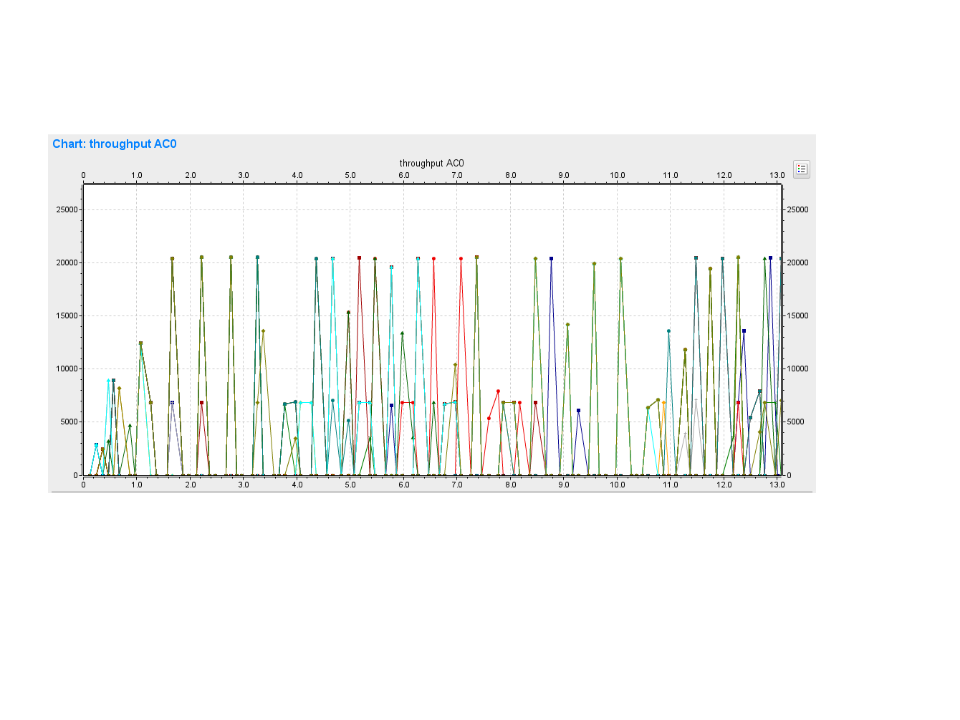
\includegraphics[width=90mm]{figs/Baseline_Omnet.png}
        \caption{Baseline OMNeT Throughput}
        \label{fig:BaselineOMNeT}        
\end{figure}

The above figure represents the throughput of the entire network. You can see from the Network results the periodic nature of the sensors where many packets are sent at the same time frame. This corresponds to the sensors periodic data packets being sent out. Due to the nature of OMNeT simulations we have all sensors sending data at once, thus the high peaks. To increase the realistic nature in the future having the sensors start time set as a randomly within the first few seconds of the simulation would increase the realistic nature of the simulation. 

\begin{figure}[ht!]
        \centering
		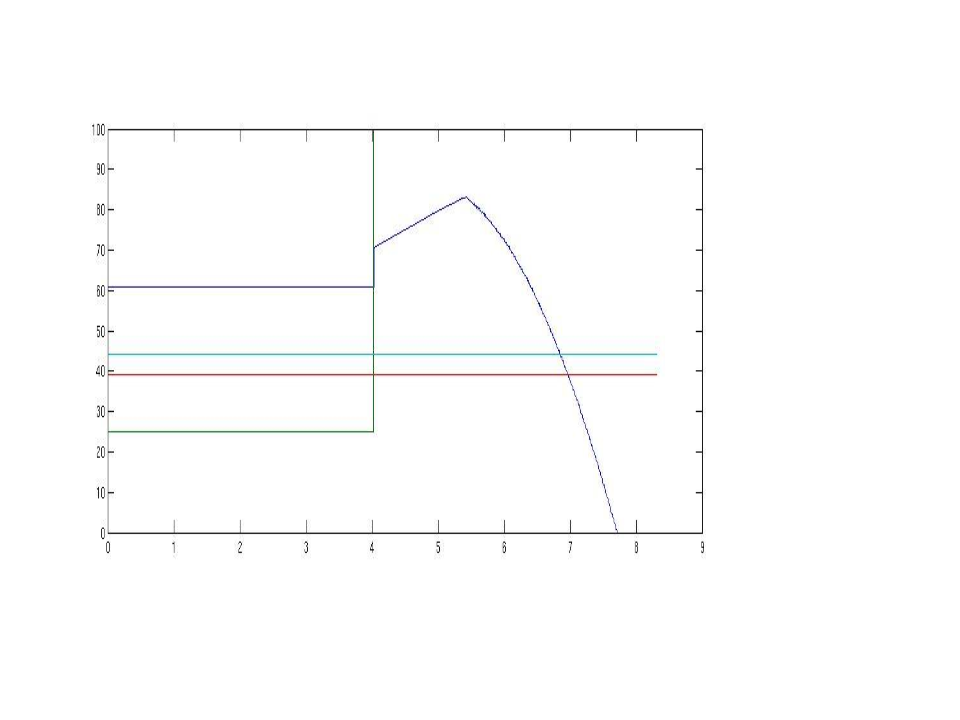
\includegraphics[width=90mm]{figs/Baselin_Matlab_control.png}
        \caption{Baseline MATLAB Control Variables}
        \label{fig:BaselineMATLABControl}        
\end{figure}

\begin{figure}[ht!]
        \centering
		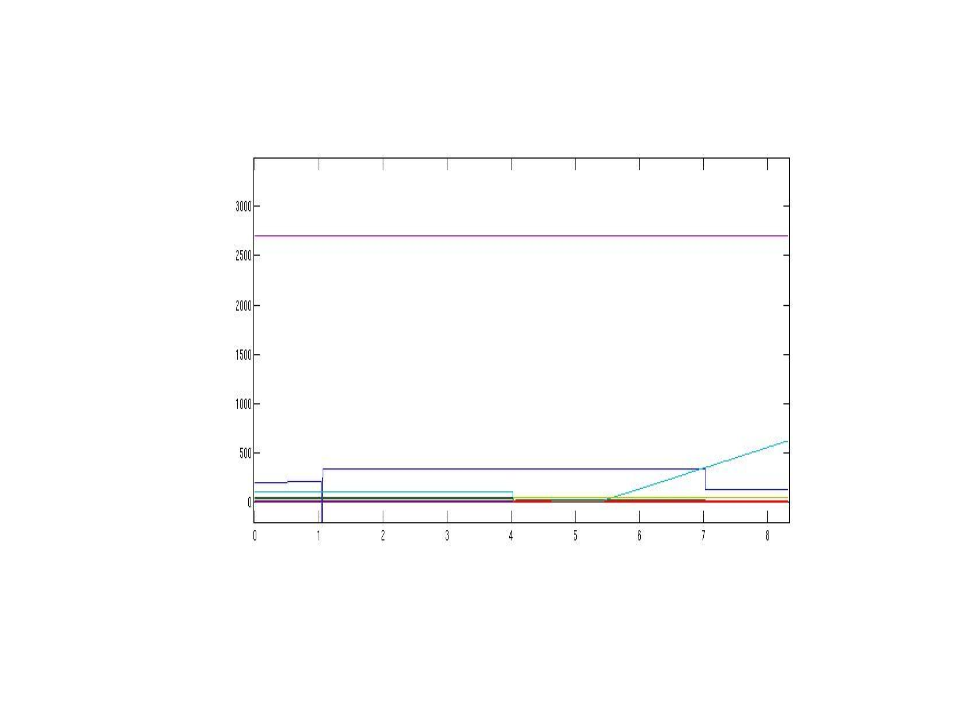
\includegraphics[width=90mm]{figs/Baseline_Matlab_sensors.png}
        \caption{Baseline MATLAB Sensor Variables}
        \label{fig:BaselineMATLABSensors}        
\end{figure}

Both of these results show the MATLAB side of the simulation. The control system adjusts the inputs until the system will arrive at a steady state. We also see the gradual nature of the controller which, in later examples is destroyed by attacks. 

\subsection{DDoS}

For our fist and most basic attack we did a simple denial of service attack, not allowing any packets from the wireless side of the network to pass through. Thus, while the controller sent quite a bit of data, it was never received by the actuators and the sensor data never got to the controller. 

\begin{figure}[ht!]
        \centering
		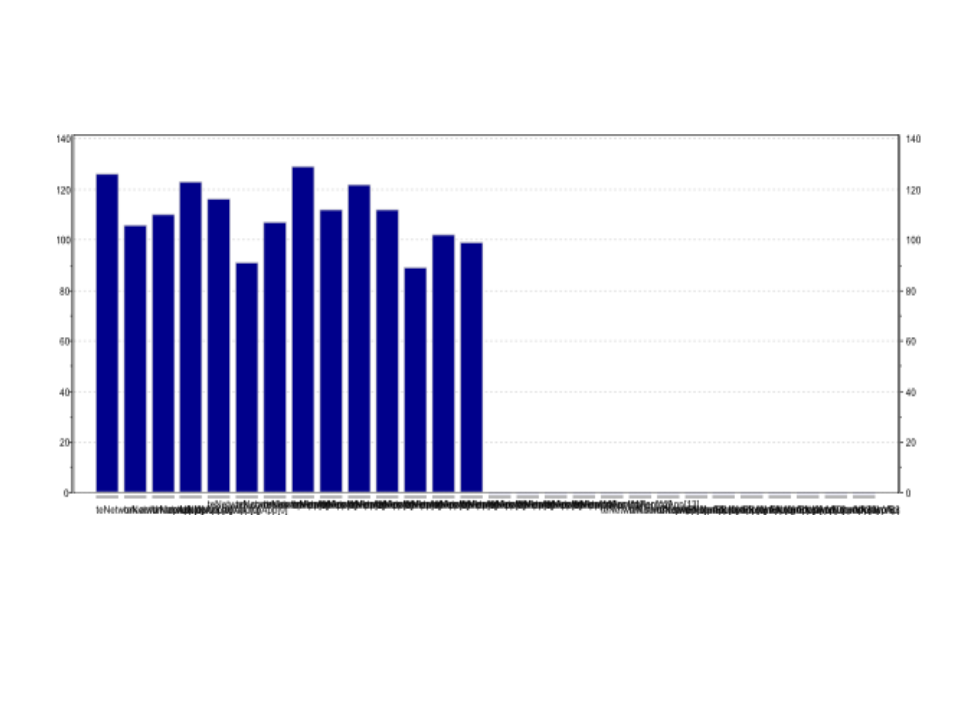
\includegraphics[width=90mm]{figs/DOS_Omnet.png}
        \caption{DOS Omnet Packets (10s simulation time)}
        \label{fig:DOSOmnetThroughput}        
\end{figure}

The right hand side of this graph shows that only ~100 packets were transmitted when, in a normal system due to the 10ms refresh rate it should look more like 100s. In this attack we successfully break the MATLAB simulation. More results of that that looks like is shown below. 

\subsection{Spoofing}

The last attack we work on was based on a malicious module that would send out false packets of data, essentially holding one value of the simulation constant and not allowing the controlled to change the value. As show below this can cause the matlab simulation to fail completely. It should also be noted that currents the sensors, actuators and controller has no notion of an "emergency shutdown" and so errors tend to accumulate and thus create no realistic results. 

\begin{figure}[ht!]
        \centering
		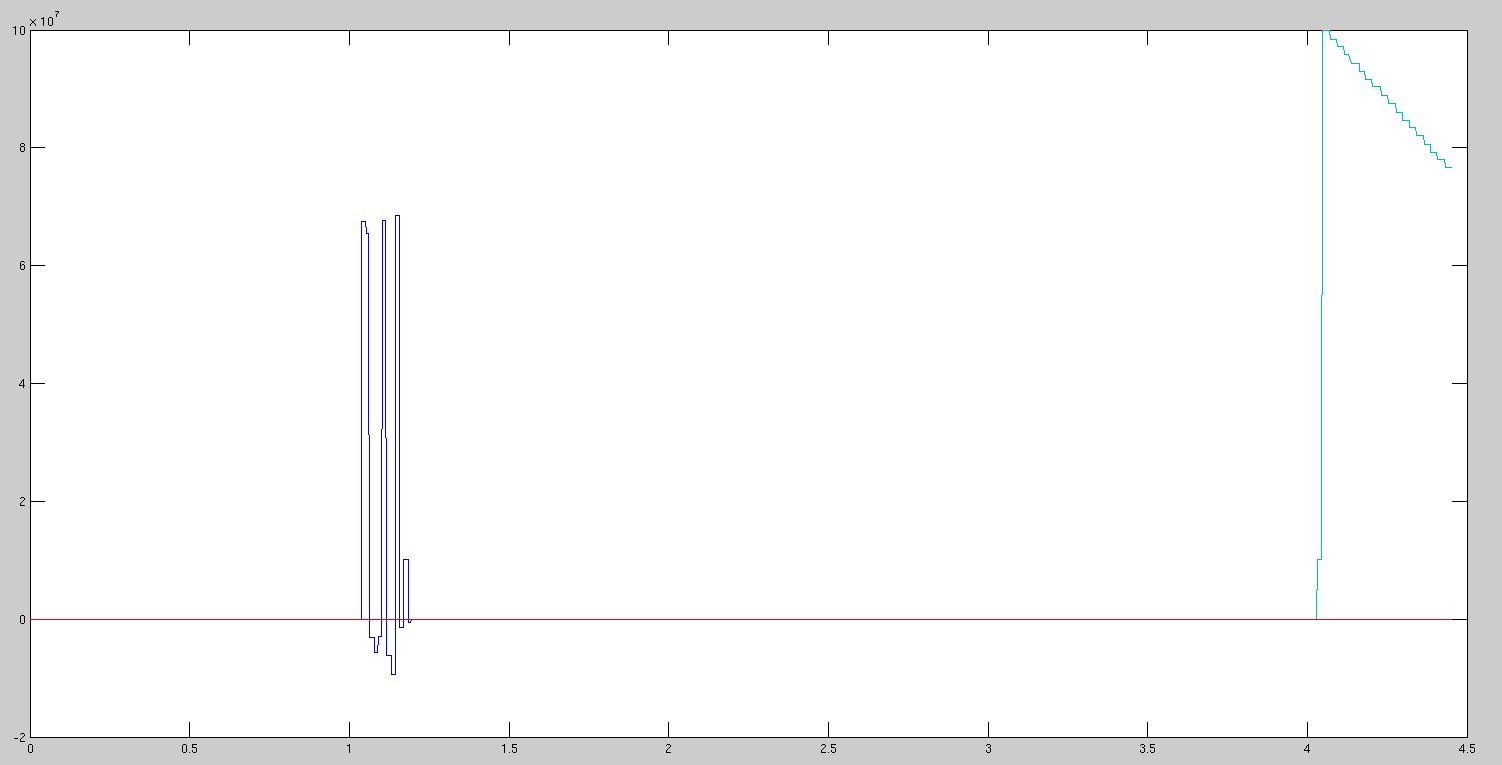
\includegraphics[width=90mm]{figs/broken_outputs.jpeg}
        \caption{Spoofing MATLAB Controller Outputs}
        \label{fig:SpoofingAttackActuators}        
\end{figure}

\begin{figure}[ht!]
        \centering
		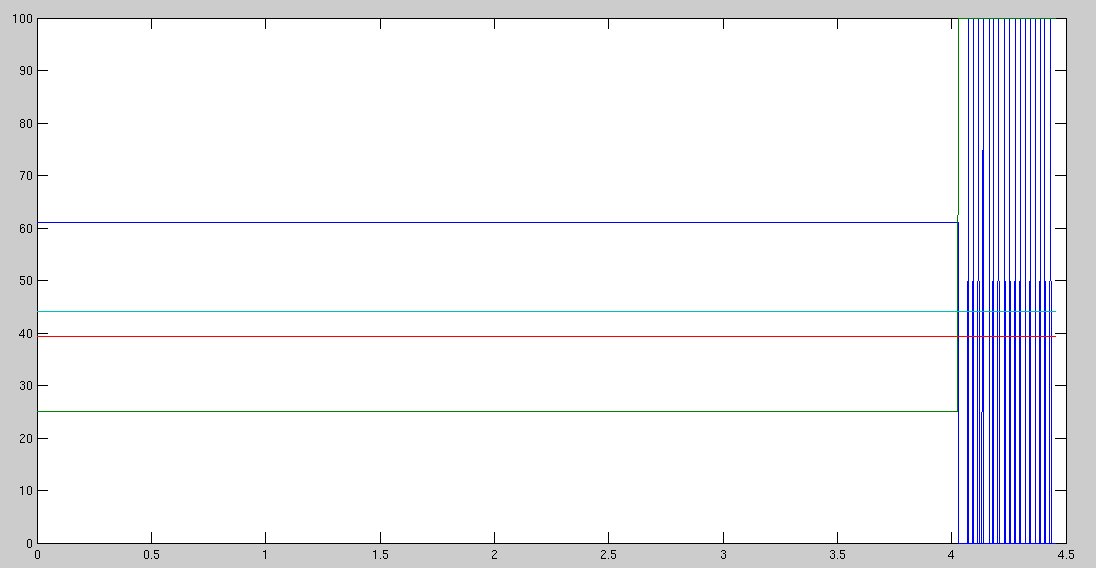
\includegraphics[width=90mm]{figs/broken_inputs.jpeg}
        \caption{Spoofing MATLAB Sensor Values}
        \label{fig:SpoofingAttackSensors}        
\end{figure}



